\documentclass[11pt,compress,t,notes=noshow, xcolor=table]{beamer}


\input{../../style/preamble}
\input{../../latex-math/basic-math}
\input{../../latex-math/basic-ml}


\setbeamersize{text margin left=0.3cm,text margin right=0.3cm}


\title{Applied Machine Learning}
% \author{LMU}
%\institute{\href{https://compstat-lmu.github.io/lecture_iml/}{compstat-lmu.github.io/lecture\_iml}}
\date{}

\begin{document}

% TODO add a title figure
\titlemeta{
Time Series:
}{
Definition, feature engineering, cross-validation
}{
figure_man/empty
}{
\item What is a time series?
\item Important definitions
\item Feature engineering for time series
\item Time series cross-validation
}


\begin{vbframe}{Running Example: The Bike Sharing Dataset}
\vfill
Hourly bike rental data from Washington D.C.
\vfill
\small % otherwise the last column does not fit
\begin{tabular}{llllrrrrlr}
\toprule
 & holiday & workingday & weather & temp & feel\_temp & humidity & windspeed & datetime & count \\
\midrule
0 & False & False & clear & 9.84 & 14.395 & 0.81 & 0.00 & 2011-01-01 00:00:00 & 16 \\
1 & False & False & clear & 9.02 & 13.635 & 0.80 & 0.00 & 2011-01-01 01:00:00 & 40 \\
2 & False & False & clear & 9.02 & 13.635 & 0.80 & 0.00 & 2011-01-01 02:00:00 & 32 \\
3 & False & False & clear & 9.84 & 14.395 & 0.75 & 0.00 & 2011-01-01 03:00:00 & 13 \\
4 & False & False & clear & 9.84 & 14.395 & 0.75 & 0.00 & 2011-01-01 04:00:00 & 1 \\
\bottomrule
\end{tabular}
\vfill
\pause
Task: Predict hourly rental count
\pause
Question: how to feed this to a standard ML model?
\vfill
\end{vbframe}


\begin{vbframe}{Key Definitions}
  \begin{itemize}
    \item \textbf{Time series} $\{y_t\}_{t=1}^{T}$: ordered observations indexed by time:
    \begin{itemize}
        \item Timestamps - Specific instants in time.
        \item Fixed periods - Such as the whole month of January 2017, or the whole year 2020.
        \item Intervals of time - Indicated by a start and end timestamp. Periods can be thought of as special cases of intervals.
        \item Experiment or elapsed time - Each timestamp is a measure of time relative to a particular start time (e.g., the diameter of a cookie baking each second since being placed in the oven), starting from 0.
    \end{itemize}
    \item \textbf{Exogenous variable / covariate}: external feature $x^{(j)}_t$ influencing $y_t$
    \item \textbf{Trend}: long-term increase or decrease
    \item \textbf{Seasonality}: systematic, calendar-related patterns
    \item \textbf{Stationarity} (briefly): distribution of $y_t$ does not change over time
  \end{itemize}
\end{vbframe}

\begin{vbframe}{Tasks}
\vfill
    \begin{itemize}
        \item Time Series Analysis
        Decompose time series into trends for understanding $\rightarrow$ time series course
        
        \item Time Series Forecasting

        Fit a model on historical data and make predictions about the future.
        \item Time Series Classification

        Make predictions about one complete time series, e.g., one recording of an experiment.
    \end{itemize}
\vfill
\end{vbframe}

\begin{vbframe}{How to tackle time series?}
\vfill
    \begin{itemize}
        \item Statistical Models
        ARIMA (Autoregressive integrated moving average) and ETS (Error, Trend, Seasonality) $\rightarrow$ time series course
        
        \item Recurrent Models

        Deep learning architectures that track the state of data over time $\rightarrow$ part of the deep learning lecture

        \item Transformer Models

        Deep learning architecture that can treat series data in an auto-regressive manner $\rightarrow$ part of the deep learning lecture
        
        \item Feature Engineering for Machine Learning

        Make predictions about one complete time series, e.g., one recording of an experiment.
    \end{itemize}
\vfill
\end{vbframe}

% =========================================================
\section{Time-Series Cross-Validation}
% ---------------------------------------------------------
\begin{vbframe}{Chronology-Aware Splits}
  \begin{figure}[h]
    \centering
        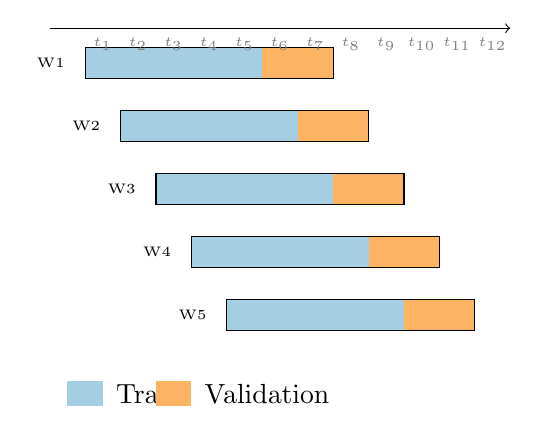
\begin{tikzpicture}[x=0.45cm,y=0.8cm]
      % Color definitions
      \definecolor{train}{RGB}{166,206,227}  % light blue
      \definecolor{val}{RGB}{253,180,98}     % light orange

      % Helper macro  {window index}{y-offset}{train start}{val start}{val end}
      \newcommand{\window}[5]{%
        % Train rectangle
        \fill[train] (#3,#2) rectangle (#4,#2+0.5);
        % Validation rectangle
        \fill[val] (#4,#2) rectangle (#5,#2+0.5);
        % Outline
        \draw (#3,#2) rectangle (#5,#2+0.5);
        % Label
        \node[left] at (#3-0.3,#2+0.25) {\tiny W#1};}

      % Five windows (progressively rolling forward)
      %            idx y   trainStart valStart valEnd
      \window{1}{0}{1}{6}{8}
      \window{2}{-1}{2}{7}{9}
      \window{3}{-2}{3}{8}{10}
      \window{4}{-3}{4}{9}{11}
      \window{5}{-4}{5}{10}{12}

      % Horizontal timeline for reference
      \draw[->] (0,0.8) -- (13,0.8);
      \foreach \t in {1,...,12} {
        \node[below,gray] at (\t+0.5,0.8) {\tiny $t_{\t}$};}

      % Legend
      \fill[train] (0.5,-5.2) rectangle (1.5,-4.8);
      \node[right] at (1.6,-5) {Train};
      \fill[val] (3,-5.2) rectangle (4,-4.8);
      \node[right] at (4.1,-5) {Validation};
    \end{tikzpicture}
  \end{figure}
  \begin{itemize}
    \item \textbf{Expanding window}: grow train set, roll validation forward
    \item \textbf{Sliding window}: fixed-width train and validation segments
    \item Validation window should match the application forecasting windows
  \end{itemize}
\end{vbframe}

\begin{vbframe}{Avoiding Data Leakage}
\vfill
  \begin{itemize}
    \item Compute lagged / rolling features \emph{after} defining the split or in a way it takes the split into account
    \item No peeking into future data when standardizing / scaling
    \item Requires special cross-validation methods
  \end{itemize}
\vfill
\end{vbframe}

\begin{vbframe}{Evaluation Metrics}
\vfill
  \begin{itemize}
    \item \textbf{MAE} $= \frac{1}{n}\sum |y_t-\hat y_t|$ (robust to outliers)
    \item \textbf{RMSE} (penalizes large errors)
    \item \textbf{SMAPE}: symmetric MAPE avoids division issues when $y_t$ near 0
    \begin{itemize}
        \item Symmetric Mean Absolute Percentage Error
        \item ${\text{SMAPE}}={\frac {100}{n}}\sum _{t=1}^{n}{\frac {|F_{t}-A_{t}|}{|A_{t}|+|F_{t}|}}$
    \end{itemize}
  \end{itemize}
\vfill
\end{vbframe}

\begin{vbframe}{Simple Baseline}
% \pause
\large
\vfill
  $y_{t+1} = y_t$
\vfill
\end{vbframe}

% =========================================================
\section{Feature Engineering}
% ---------------------------------------------------------
\begin{vbframe}{Calendar Features}
  \vfill
  \begin{itemize}
    \item Day-of-Week, Day-of-Month, Week Number, Month, Quarter
    \item Boolean flags: public holidays, weekend, promotion days, end-of-month
  \end{itemize}
  \vspace{0.4cm}
  \begin{block}{Why?}
    Capture human or process-driven periodicity.
  \end{block}
  \vfill
  \pause
  Caveat: pay attention to the calendar if the events do not follow the Gregorian calendar
  \vfill
\end{vbframe}

\begin{vbframe}{Cyclic Encoding}
  \vfill
  \[\text{sin}(2\pi \tfrac{hour}{24}),\; \text{cos}(2\pi \tfrac{hour}{24})\]
  \vfill
  \begin{itemize}
    \item Converts periodic integers (hour 0-23, month 1-12) into continuous space
    \item Eliminates artificial jump between 23 \(\rightarrow\) 0
  \end{itemize}
  \vfill
\end{vbframe}

\begin{frame}{Cyclic Encoding Visualization (Hour 0-23)}
  \begin{figure}
    \centering
    \begin{tikzpicture}[scale=2]
      % Axes
      \draw[->] (-1.2,0) -- (1.25,0) node[right] {$\cos(2\pi h/24)$};
      \draw[->] (0,-1.2) -- (0,1.25) node[above] {$\sin(2\pi h/24)$};
      % Unit circle
      \draw[gray!60] (0,0) circle (1);
      % Hour points
      \foreach \h in {0,...,23}{
        \coordinate (p) at ({cos(90-\h*15)},{sin(90-\h*15)});
        \fill[blue!70] (p) circle (1.3pt);
        \node[font=\tiny] at ($1.15*(p)$) {\h};
      }
    \end{tikzpicture}
  \end{figure}
\end{frame}

\begin{vbframe}{Lagged \& Auto-Regressive Features}
  \vfill
  \begin{itemize}
    \item Plain lags: $y_{t-1},\;y_{t-7},\;y_{t-14}$
    \item Multi-step: include future-known covariates (e.g., planned price)
    \item Combine with calendar features for interactions
  \end{itemize}
  \vfill
  \pause
\begin{tabular}{llrrrrr}
\toprule
 & datetime & count & lag\_168 & lag\_336 & lag\_504 & lag\_672 \\
\midrule
17374 & 2012-12-31 19:00:00 & 119 & 18 & 507 & 564 & 692 \\
17375 & 2012-12-31 20:00:00 & 89 & 23 & 340 & 427 & 471 \\
17376 & 2012-12-31 21:00:00 & 90 & 22 & 200 & 300 & 300 \\
17377 & 2012-12-31 22:00:00 & 61 & 12 & 120 & 245 & 221 \\
17378 & 2012-12-31 23:00:00 & 49 & 11 & 54 & 126 & 144 \\
\bottomrule
\end{tabular}
\vfill
\end{vbframe}

\begin{vbframe}{Rolling / Expanding Statistics}
  \vfill
  \begin{itemize}
    \item Rolling mean / std / min / max over window
    \item Expanding mean: trend indicator
    \item Percentiles: 25th, 75th for distribution shape
  \end{itemize}
  \vfill
\end{vbframe}

\begin{vbframe}{Interaction Features}
  \vfill
  \begin{itemize}
    \item Lag $\times$ Holiday flag
    \item Weather $\times$ Weekend indicator
    \item Captures non-linear, conditional effects
  \end{itemize}
  \vfill
\end{vbframe}

% =========================================================
\section{Wrap-Up}
% ---------------------------------------------------------
\begin{vbframe}{Key Takeaways}
  \vfill
  \begin{itemize}
    \item Feature engineering often outweighs model complexity in time-series ML.
    \item Use chronology-aware CV to obtain honest performance estimates.
    \item Always benchmark against a naive or seasonal naive baseline.
  \end{itemize}
  \vfill
\end{vbframe}


\endlecture
\end{document}

